\documentclass[a4paper,12pt, openany]{jsbook}

\usepackage{enumerate}
\usepackage{paralist}

\usepackage{graphicx}


% theorem
\usepackage{amsmath,amssymb}
\usepackage{amsthm}
\makeatletter
\renewenvironment{proof}[1][\proofname]{\par
  \pushQED{\qed}%
  \normalfont \topsep.5\baselineskip \labelsep1zw
  \trivlist
  \item[\hskip\labelsep
        \textsf{#1}]\ignorespaces
}{%
  \popQED\endtrivlist\@endpefalse
}
\makeatother
\renewcommand{\proofname}{証明}


% Tikz
\usepackage[dvipdfmx,svgnames]{xcolor}
\usepackage{tikz}

\def\newblock{\hskip .11em plus .33em minus .07em}

\newcommand{\figdir}{../figures}
\newcommand{\ncomment}[1] {{\textcolor{red}{#1}}}
\newcommand{\kcomment}[1]{{\textcolor{blue}{#1}}}


\newcommand{\independentPatProb}{《独立警邏問題》}
\newcommand{\patProb}{《警邏問題》}
\newcommand{\timeSpecifiedPatProb}{時刻指定警邏問題}
\newcommand{\timeSpecifiedPatProbDecision}{時刻指定警邏判定問題}
\newcommand{\timeSpecifiedPatProbOnLine}{時刻指定線分警邏判定問題}
\newcommand{\setPartitionAlgorithm}{分割アルゴリズム}
\newcommand{\intervalSpecifiedPatProb}{間隔指定警邏問題}
\newcommand{\intervalSpecifiedPatProbDecision}{間隔指定警邏判定問題}

\newcommand{\idletime}{《訪問間隔上限》}
\newcommand{\exactIdletime}{《指定時刻》}
\newcommand{\exactInterval}{訪問間隔}
\newcommand{\indSectOperation}{独立往復運行}
\newcommand{\graphLine}{Line}
\newcommand{\graphStar}{Star}
\newcommand{\graphUnit}{Unit}



\newcommand{\Rset}{\mathbf R}
\newcommand{\Nset}{\mathbf N}
\newcommand{\Zset}{\mathbf Z}
\newcommand{\abs}[1]{\lvert{#1}\rvert}
\newcommand{\card}[1]{\lvert{#1}\rvert}



%%%%% 定理環境 %%%%%
\theoremstyle{definition}
\newtheorem {theo}          {定理}[section]
\newtheorem {defi}[theo]    {定義}
\newtheorem {prop}[theo]    {命題}
\newtheorem {lemm}[theo]    {補題}
\newtheorem {coro}[theo]    {系} % corollary
\newtheorem {conj}[theo]    {予想} % conjecture
\newtheorem*{rema}          {Remark}
\newtheorem*{exam}          {例}
\newtheorem*{property}      {性質}

\newtheorem*{patrollingProblem}{{\patProb}}
\newtheorem*{timeSpecifiedPatrollingProblem}{{\timeSpecifiedPatProb}}
\newtheorem*{timeSpecifiedPatrollingProblemDecision}{{\timeSpecifiedPatProbDecision}}
\newtheorem*{timeSpecifiedPatrollingProblemOnLine}{{\timeSpecifiedPatProbOnLine}}
\newtheorem*{setPartitionAlgorithmForTimeSpecifiedProblemOnLine}{{\setPartitionAlgorithm}}
\newtheorem*{intervalSpecifiedPatrollingProblemDecision}{{\intervalSpecifiedPatProbDecision}}



\begin{document}

  \begin{center}
    {\LARGE 修士学位論文} \par
    \vfill
    {\LARGE 複数の巡査の協力による指定地点の警邏について} \\
    {\normalsize Collaborative Patrolling of Designated Points on Graphs} \par
    \vfill
    {\large
    2017年度 \\
    広域科学専攻・広域システム科学系 \\
    31-166813 \\
    能城秀彬
    }
  \end{center}
  \thispagestyle{empty}  % ページ番号消去
  \clearpage

  \frontmatter
  \tableofcontents

  \mainmatter

  [最終変更日時:
{\the\year/\the\month/\the\day, {\the\hour} 時{\the\minute}分}]

 [ToDo]
\begin{itemize}
  \item \textbf{図の追加・差し替え}
  \item 最終チェック
  \begin{itemize}
    \item 並列列挙は・で
    % \item 補足(不要?)
    % \begin{itemize}
    %   \item \ref{theo:LineUnaryIdletimePolyTimeSolvable}
    %     各区間の利得の計算や選ばれた区間に含まれる点の列挙の方法
    %   \item \ref{section:LineArbitraryIdletime}節:
    %     運行可能集合$S$に対して運行$a$が存在することの証明
    % \end{itemize}
  \end{itemize}
\end{itemize}

  \section{はじめに}
\label{section: introduction}
所与の領域を一人または複数の巡査が動き回り,
その領域内の指定された場所を十分な頻度で訪れることを
警邏(patrolling)という\cite{chen2013fence, coene2011charlemagne, czyzowicz2011boundary}.
\ncomment{[警邏問題を代表するにふさわしい文献を]}

本稿では,与えられた距離空間$U$内を速さ$1$以下の巡査$m$人が動きまわることにより,
集合$V \subseteq U$に属する多くの点に十分な頻度で訪れるという目標を考える.
すなわち次のような問題である.

巡査$i \in \{1, \ldots, m\}$の$U$上の運行$a _i \colon \Rset \to U$とは,
各時刻$t \in \Rset$における位置$a _i (t) \in U$を定めるものであって,
任意の時刻$s$,$t \in \Rset$に対し$a _i (s)$と$a _i (t)$の距離が$\abs{s - t}$を超えないものをいう.
巡査$m$人による$U$上の運行とは,
全巡査の運行を定めた組$A = (a _1, \dots, a _m)$をいう.
$U$の有限な部分集合$V$があり,$V$の各点には利得および{\maxIdletime}と呼ばれる正整数が定まっている.
運行$A = (a _1, \dots, a _m)$が点$v \in V$を{\maxIdletime}$q > 0$で警備するとは,
長さ$q$のどの時間区間にも
いずれかの巡査が$v$を少なくとも一度は訪れる
(任意の時刻$t \in \Rset$に対して
巡査$i$と時刻$\tau \in [t, t + q)$が存在し$a _i (\tau) = v$)
ことをいう.
運行$A$が点集合$W \subseteq V$を警邏するとは,
各点$v \in W$に対し$A$が$v$を警備することをいう.
そのような運行が存在するとき$W$は$m$人により警邏可能であるという.

\begin{patrollingProblem}
巡査の人数$m \in \Nset$と距離空間$U$内の点集合$V$および
$V$の各点の利得と{\maxIdletime}が与えられる.
$m$人の巡査により警邏可能な$V$の部分集合のうち
利得の和が最大となるものを求めよ.
\end{patrollingProblem}

距離空間$U$といっても,$V$の点同士の測地距離のみが重要である.
そこでこの問題の入力は,
$V$を頂点集合とし辺に非負整数の長さがついた無向グラフと考えることにする.

この問題は,巡査が一人かつ
全点の利得と{\maxIdletime}が等しい場合に限っても,
ハミルトン路問題からの帰着により
NP困難である\cite[Theorem~8]{coene2011charlemagne}.
そこでグラフの形状を限ったときにどのようになるかを調べる.

一つの頂点が複数の巡査の訪問により警備され得ることに注意されたい.
例えば図\ref{figure: cooperative}左はそのような運行の例である.
\begin{figure}
  \begin{center}
    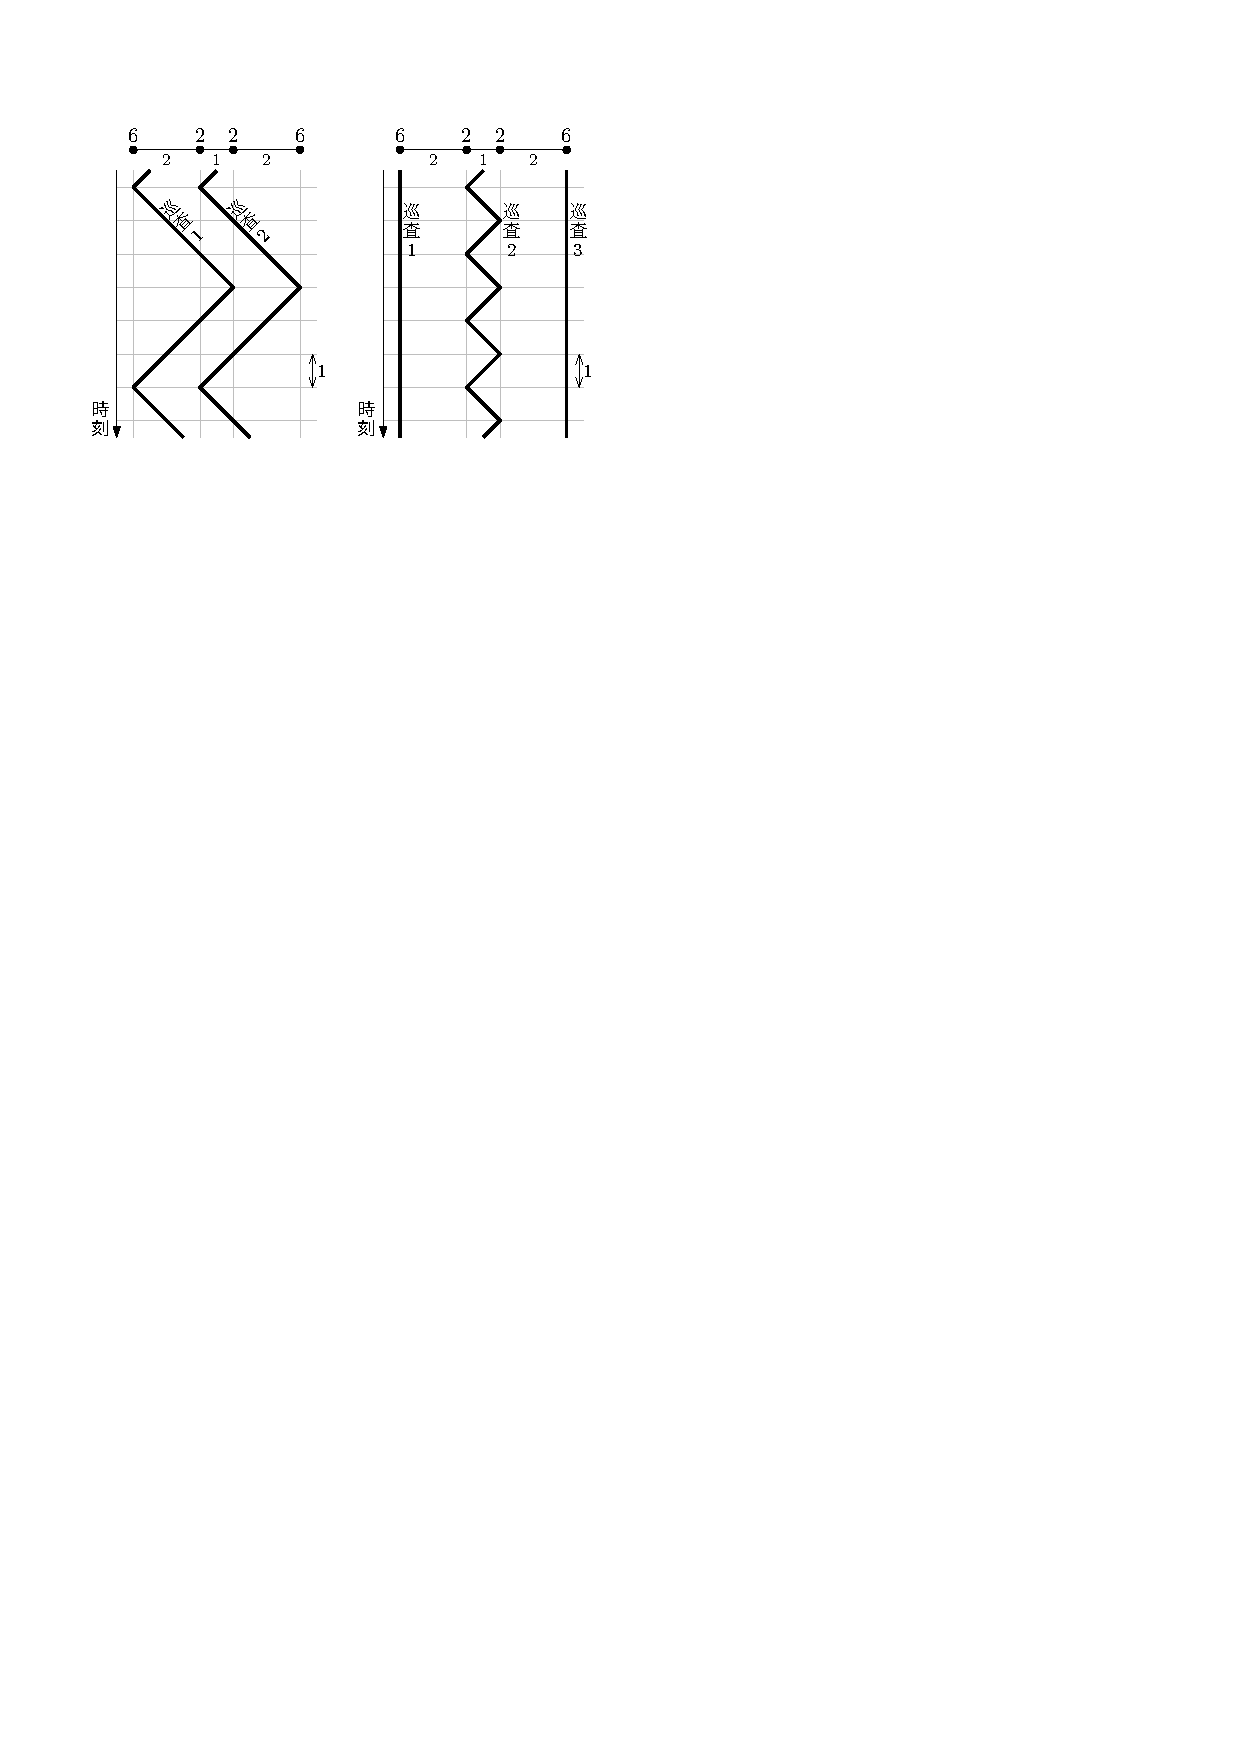
\includegraphics[scale=1.0]{\figdir/cooperative.pdf}
    \caption{図の上部に描かれている四点からなるグラフの全点を警邏する二つの運行.
      頂点と辺に書かれた数は,それぞれ{\maxIdletime}と距離である.
      左図の運行では二人の巡査が協力して中央の二点を間隔$2$で警備している.
      これを禁じ,各点がいずれかの巡査により単独警備されることを求める場合は,
      右図のように三人の巡査を要する.}
    \label{figure: cooperative}
  \end{center}
\end{figure}
Coeneら\cite{coene2011charlemagne}は似た問題を扱っているが,
このような協力を許さず,
図\ref{figure: cooperative}右のように
各頂点を専ら一人の巡査が「担当」することを要求している.
つまり,各頂点$v \in W$が単独警備される(すなわち
或る一人の巡査がおり,
その巡査のみの運行が$\{v\}$を警邏する)ことを要求しているのである.
対比のため本稿ではこの問題を{\independentPatProb}と呼ぶことにする
(\cite{coene2011charlemagne}ではMPLPPと称している).
Coeneら\cite{coene2011charlemagne}の諸結果においては,
この単独警備という限定が,
多項式時間算法の設計にも困難性の証明にも重要な役割を果している.
この限定を外したときの様子を調べるのが本稿の目的である.

本稿ではグラフの形状として
線分,星と,すべての枝の長さが等しい完全グラフの3種類を扱うこととし
(図\ref{figure: graph_classes}),
以降はそれぞれを {\graphLine}, {\graphStar}, {\graphUnit}と呼ぶ.
\begin{figure}
  \begin{center}
    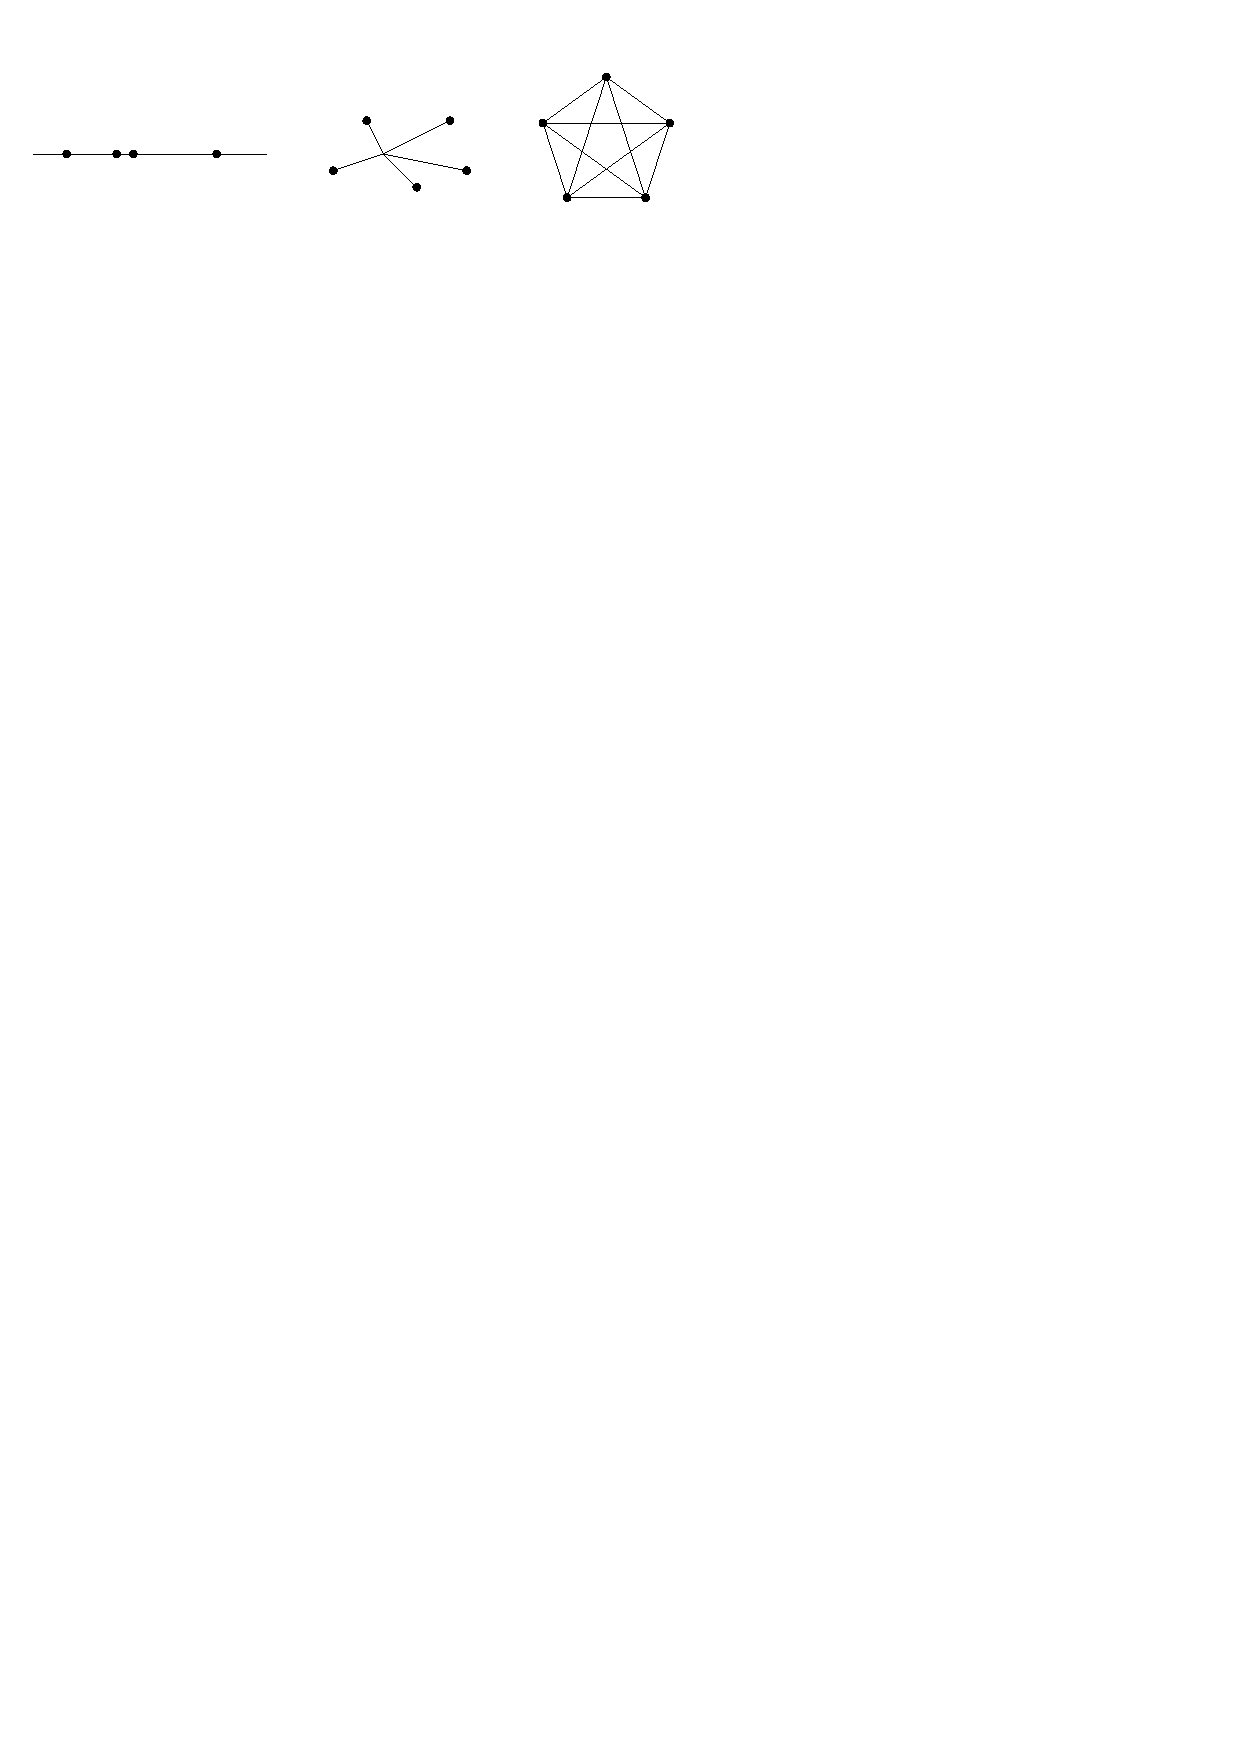
\includegraphics[scale=1.0]{\figdir/graph_classes.pdf}
    \caption{本論文では{\graphLine}(左),{\graphStar}(中),{\graphUnit}(右,但し各辺の長さが等しい)を扱う.{\graphStar}は葉のみを警備の対象とする(中央の点は移動の途中で使うのみであり,{\maxIdletime}は定められていない).}
    \label{figure: graph_classes}
  \end{center}
\end{figure}
{\graphStar}では葉のみに{\maxIdletime}が定められている(中心は警備の対象としない).
% {\patProb}においては頂点同士の測地距離のみが重要であるため,
辺の長さがすべて$d$である{\graphUnit}のグラフは
同じ頂点数で辺の長さがすべて$d/2$である{\graphStar}のグラフの場合に帰着できることから,
{\graphUnit}は{\graphStar}の特殊な場合である.


{\patProb}についての我々の結果を
Coeneらの{\independentPatProb}についての結果との比較も含めて
グラフの形ごとにまとめると次のようになる.
それぞれ\ref{section: line},\ref{section: star},\ref{section: unit}節で述べる.
\begin{itemize}
\item 
  グラフが{\graphLine}の場合は,
  {\independentPatProb}は動的計画法により多項式時間で解けることが
  示されていた\cite[Theorem~11]{coene2011charlemagne}が,
  その正しさは単独警備という設定に強く依存している.
  本稿では{\patProb}について,
  全点の{\maxIdletime}が等しい場合には多項式時間で解けることを示す
  (定理\ref{theo:LineEqualTimelimit}).
\item
  グラフが{\graphStar}の場合は,
  全点の利得と{\maxIdletime}が等しい場合に限っても,
  {\independentPatProb}はNP困難であることが示されていた\cite[Theorem~10]{coene2011charlemagne}.
  本稿では,この場合の{\patProb}は多項式時間で解けるという興味深い結果を得る(定理\ref{theo:StarEqualProfitTimelimit}).
  なお利得または{\maxIdletime}を一般にすると,
  巡査が一人であっても(したがって独立かどうかによらず)
  NP困難であることがわかっている\cite[Theorems 5 and 6]{coene2011charlemagne}.
\item 
  グラフが{\graphUnit}の場合は,
  % {\independentPatProb}では
  % 巡査が一人で利得がすべて等しく{\maxIdletime}が一般の場合は
  % 多項式時間で解けることが示されていた\cite[Theorem~7]{coene2011charlemagne}.
  % \ncomment{[{\independentPatProb}との比較と言っているので書くべきかと思ったが正しい結果でない可能性があるのであとで確認する]}
  本稿では全点の{\maxIdletime}が等しい場合は{\patProb}が多項式時間で解けることを示す(定理\ref{theo:UnitEqualTimelimit}).
  グラフが{\graphStar}の場合は全点の{\maxIdletime}が等しくても利得が一般だとNP困難になるので,
  これにより{\graphUnit}は{\graphStar}よりも簡単に解ける場合となっていることが分かる.
\end{itemize}


{\graphLine}と{\graphUnit}については
{\maxIdletime}が一般の場合については多項式時間アルゴリズムやNP困難性を示すのが難しく未解決である.
これらの未解決な状況については,
{\maxIdletime}の代わりに{\exactIdletime}を警備の条件とする次のような問題を考えた.

\begin{defi}
運行$A = (a _1, \ldots, a _m)$が点$v \in U$を
{\exactIdletime}$(q, r) \in \Nset \times \Nset$で警備するとは,
任意の時刻$t := q k + r\ (k \in \Zset)$に対し
巡査$i$が存在し$a _i (t) = v$であることをいう.
\end{defi}

\begin{timeSpecifiedPatrollingProblem}
巡査の人数$m$と距離空間$U$内の点集合$V$および各点の利得,
警備の条件として{\exactIdletime}が与えられる.
$m$人の巡査により警邏可能な$V$の部分集合のうち
利得の和が最大となるものを求めよ.
\end{timeSpecifiedPatrollingProblem}

\begin{timeSpecifiedPatrollingProblemDecision}
巡査の人数$m$と距離空間$U$内の点集合$V$および
警備の条件として各点の{\exactIdletime}が与えられる.
$m$人の巡査により$V$を警邏可能か判定せよ.
\end{timeSpecifiedPatrollingProblemDecision}


{\graphLine}については{\timeSpecifiedPatProbDecision}を解く貪欲アルゴリズムを示す(定理\ref{theo:LineTimeSpecifiedGreedy}).
{\graphUnit}については{\timeSpecifiedPatProb}がNP困難であることを示す(定理\ref{theo:unit_exacidletime_NPhard}).

  \subsection*{関連研究}
% 与えられた領域内に幾人かの巡査をうまく配置することを目的とする問題
警邏に関する問題には様々な設定が考えられている.

[メモ]
\begin{itemize}
  \item {\patProb}を考える動機
  \begin{itemize}
    \item 巡査が障害物を含む2次元平面内を動き回り警備するという目的の問題において,障害物を含む2次元平面をグラフに簡略化して考えるというところから,グラフの頂点を警備するという問題が考えられていた~\cite{machado2002multi}.
    \item (なぜ図形として{\graphLine}, {\graphStar}, {\graphUnit}を考えたか?) → {\graphLine}は塀の警邏などの文脈でよく現れるため.{\graphStar}は高さが$1$の木であり,グラフが木である場合の{\patProb}の困難性の評価のために導入した図形である.
    \item (なぜ{\maxIdletime}を警備の条件にしたか?)→ Coeneらの先行研究と似た設定を考えたかったため(自然な条件なのであまり説明しなくてよさそう?)
    \item 頂点を通過するだけで警備したことになる設定だが,より一般的に時間$d \geq 0$滞在しなければならないとしたらどうか? → 点$p$を警備するのに時間$d$滞在しなければならないとすると,$p$から長さ$d/2$の辺を伸ばした先の点$p'$を代わりに警備対象とすればよい.
    \item 
    \item 
  \end{itemize}

  \item 問題設定の大枠について
  \begin{itemize}
    \item 現実の警備の問題としては,警備の仕方として領域内を巡査動き回るというものの他にも,領域の周囲を巡回するという警備の仕方も考えられる.実際に塀の警邏問題として知られている~\cite{czyzowicz2011boundary, dumitrescu2014fence, kawamura2015fence}.
    \begin{itemize}
      \item 一次元の連続領域のすべての点が警備対象
      \item 線分や閉路の一部のみが警備対象であるという中間的な問題設定も考えられている~\cite{collins2013optimal}.警備対象を有限個の点とすると{\patProb}と似た問題になり,警備対象を全体とすると塀の警邏問題と似た問題となる.
    \end{itemize}
    \item {\patProb}では,{\maxIdletime}の条件さえ満たしていれば警備できるという設定で考えており,侵略者の動きなどは具体的に考えていないが,侵略者の動き方まで含めてゲーム理論的に考察している研究も存在する~\cite{brazdil2015strategy, papadaki2016patrolling}.
    \item {\patProb}では,巡査達は決定論的に動くので,現実的には十分賢い侵略者に対応されてしまう欠点がある.
    巡査の運行戦略にランダム性を取り入れたものがある~\cite{}.
    \item {\patProb}では,警備対象の環境が与えられたときに最適な巡査の運行を決定してしまって巡査がその通りに動くという意味で,中央集権的な運行の決定をしているとみなすことができる.
    一方で,巡査がその近傍の情報から各々の判断で運行を決定するという設定のものも考えられている~\cite{}.
  \end{itemize}

  \item 問題に対する様々なアプローチ
  \begin{itemize}
    \item 理論的な研究を行うもの
    \item ヒューリスティックな戦略を先に与え,計算機でシミュレーションを行うもの
    \item 実際のロボットで実験しているものもある
  \end{itemize}

  \item 似た問題設定の他の研究との細かい違いについて
  \begin{itemize}
    \item 最適化する指標
    \begin{itemize}
      \item 全点警備可能な最小の巡査数を求める
      \item 警邏できる部分集合であって点の数や利得の合計が最大のものを求める
      \item 与えられた巡査により全点を警備する上で,
      各点の訪問頻度を(同程度にする・平均値を最大化する・最小の訪問頻度を最大化する)など
      \begin{itemize}
        \item 
      \end{itemize}
    \end{itemize}
    \item 巡査の速さがすべて同じであるという仮定を置いているが,異なる速さの巡査が存在する場合も調べられている~\cite{}.
  \end{itemize}

  \item その他
  \begin{itemize}
    \item 分割戦略と巡回戦略
    \begin{itemize}
      \item 多くの場合TSPに基づく巡回が最適だが,
      長い辺がある場合や巨大グラフの場合に問題がある.
      \item TSPに基づく巡回が多くの場合最適なのでTSPの解を求める近似アルゴリズムにより巡査の運行を決めるものも
    \end{itemize} 
    % \item 他にも,警備対象や巡査の動く領域が時間変化するような場合なども現実の模倣としては考えられるが,
    % 簡単化されたモデルを扱うものが多い.
    % \item {\patProb}は一般グラフではハミルトン閉路問題の帰着によりNP困難であることが知られているが,
    % 逆にTSPの解による巡回で
  \end{itemize}
\end{itemize}


% 警邏に関する研究には様々な問題設定があり,
% 例えば線分や閉路のような交わりの無い1次元的な領域のすべての点を警邏する
% 塀の警邏(Fence Patrolling)問題~\cite{chen2013fence, czyzowicz2011boundary}や,
% より一般的なグラフで辺全体ではなく頂点を警備する警邏問題~\cite{coene2011charlemagne},
% グラフと巡査が与えられて警邏可能かを判定する問題だけでなく,
% 塀の警邏問題においてなるべく長い塀を警邏する問題~\cite{czyzowicz2011boundary}や
% 全体の訪問の待ち時間の最大値を最小化する問題~\cite{chen2013fence}
% なども考えられている.

% また,{\graphLine}や{\graphStar}は木の特別な場合である.

  \section{{\graphLine}}
\label{section: line}

グラフが{\graphLine}の場合,
グラフの全体(頂点と辺)をすべて実直線上におくことができる.
以降,頂点の名前$v_1, v_2, \ldots, v_n$などはその位置の実数値も表すことにする.

{\graphLine}の場合には順序保存運行という特別な運行を考えることができる.
運行$A = (a_1, \ldots, a_m)$が順序保存であるとは,
任意の時刻$t \in \Rset$において
$a_1(t) \leq a_2(t) \leq \cdots \leq a_m(t)$を満すことである.
巡査$m$人で警邏可能な任意の頂点集合$W$に対して,
巡査$m$人の順序保存運行が存在して$W$はこれにより警邏される.
これは,
ある運行$A$により警邏される集合$W$は,
巡査の最高速度がすべて同じであることから
$A$で2人の巡査がすれ違うときに代わりに互いの以降の運行を交換し引き返すようにした運行
$A'$によっても$W$が警邏されるためである.



\subsection{全点の{\maxIdletime}が等しい場合}
\label{subsec:LineUnaryTimelimit}


本節では次のことを示す.

\begin{theo}
\label{theo:LineEqualTimelimit}
グラフの形状が{\graphLine}で全点の{\maxIdletime}が等しい場合,
{\patProb}は頂点数$n$と巡査数$m$の多項式時間で解くことができる.
\end{theo}

この場合については,全点を警備可能か判定する問題ならば
Collinsら~\cite{collins2013optimal}の問題の特殊な場合として既に示されているが,
ここでは全点の{\maxIdletime}が等しいという条件のみでも成り立つことを示す.

以降では,
グラフの形状が{\graphLine}で全点の{\maxIdletime}が等しい場合,
各巡査が部分集合を担当し独立に往復するという単純な運行によって
最大利得が得られることを示す.
以下,各頂点の{\maxIdletime}が$Q$のとき,
各巡査が$V$のいずれかの頂点を左端とする長さ$Q/2$の区間を往復する運行を{\indSectOperation}と呼ぶことにする.
また,巡査$m$人の運行$A$において各巡査が{\indSectOperation}をしているとき,
$A$を$m$人の巡査による{\indSectOperation}と呼ぶ.


\begin{lemm}
  \label{lemm:RangeOfPatrollerOnLine}
  頂点$v_i$がある一人の巡査$s$により単独警備されているとき,
  {\maxIdletime}を$q_i$として,
  $s$は常に区間$[v_i - q_i/2, v_i + q_i/2]$にいる.
\end{lemm}
\begin{proof}
  \newcommand{\vout}{v_{\mathrm{out}}}
  この区間にない或る座標$\vout \notin [v_i - q_i/2, v_i + q_i/2]$を$s$が
  時刻$t_0$に訪問するとする.
  $\vout$と$v_i$の間の移動には
  少なくとも時間$\abs{v_i - \vout} > q _i / 2$を要するから,
  $s$は区間$[t_0 - q _i / 2, t_0 + q _i / 2]$に属する時刻に$v_i$を訪問できない.
  この区間の長さは$
    q_i
  $であるので,$s$が$v _i$を単独警備していることに反する.
\end{proof}


\begin{lemm}
\label{lemm:LineEqualTimelimitIndependentInterval}
グラフの形状が{\graphLine}で,全点の{\maxIdletime}が等しいとする.
頂点集合$V$の任意の部分集合$W$に付いて、
$W$が巡査$m$人により警邏可能ならば$W$は巡査$m$人による独立往復運行で警邏できる.
\end{lemm}
\begin{proof}
\newcommand{\leftmostpoint}{b}  % v以外の記号
\newcommand{\newpatroller}{l}
\newcommand{\leftmostpatroller}{巡査1}
\newcommand{\leftmostpatOpr}{a_1}

巡査数$m$に関する帰納法で示す.
全点の{\maxIdletime}を$Q$とする.
$m = 0$のときは明らかなので,以下$m > 0$とする.

$W$は$m$人の巡査により警邏可能であるので,2節始めの議論により$W$を警邏する$m$人の巡査による順序保存運行が存在する.
このような運行を任意に一つ選び
$A = (a _1, \ldots, a _m)$
とする.

$W$の点のうち最も左にあるものを$\leftmostpoint$とする.
まず,各巡査は
$\leftmostpoint$より左に存在する時間
$\leftmostpoint$で停止するように変換する.
このようにしても$W$は警邏されたままであり,
また,これによりすべての巡査は
区間$[\leftmostpoint, +\infty)$に存在することになる.

ここで,最も左の巡査$\leftmostpatroller$に注目する.
順序保存であることから$\leftmostpoint$が$A$により訪問されるすべての時刻に
$\leftmostpatroller$は$\leftmostpoint$を訪問しているので,
$\leftmostpoint$は$\leftmostpatOpr$により単独警備されている.
%
すると,
補題\ref{lemm:RangeOfPatrollerOnLine}より,
任意の時刻$t \in \Rset$に対し
$\leftmostpatOpr(t) \leq \leftmostpoint + Q/2$
であるが,
%
一方,$\leftmostpatOpr$を区間$[b, b + Q/2]$を速さ$1$で往復する運行とすれば
この区間に含まれるすべての頂点を警備することができる.
実際,$\leftmostpatOpr$がこのような運行であるとき
$\leftmostpoint \leq x \leq \leftmostpoint + Q/2$
である位置$x$に存在する時刻の間隔の最大値は
$ \max( 2(x - \leftmostpoint), 2(\leftmostpoint + Q/2 - x) )
  \leq 2(\leftmostpoint + Q/2 - \leftmostpoint) = Q $
より,$[\leftmostpoint, \leftmostpoint + Q/2]$に含まれるどの頂点も
{\maxIdletime}を超えずに訪問できていることが分かる.
% これにより$\leftmostpatroller$の運行は{\indSectOperation}となる.
%
一方,$W^- := \{ v \in W \mid \leftmostpoint + Q/2 < v \}$は
$A$で$\leftmostpatroller$以外の$m - 1$人の巡査により警備されているので,
帰納法の仮定から残る$m - 1$人の巡査も{\indSectOperation}に変換することができる.
以上により$W$を警邏する$m$人の巡査による{\indSectOperation}が得られた.
\end{proof}


補題\ref{lemm:LineEqualTimelimitIndependentInterval}により,
{\graphLine}のグラフで全点の{\maxIdletime}が等しい場合の運行は
{\indSectOperation}のみを考えればよいため,
$I_1, \ldots, I_n$から
$m$人の巡査がそれぞれ担当する$m$個の区間のうち利得の合計が最大となるものを求めればよい.
これは以下のアルゴリズムにより求めることができる.

初めに{\graphLine}上の頂点をソートしておき,左側から順に$v_1, v_2, \ldots, v_n$とする.
頂点$v_i$を左端とする区間を$I_i := [v_i, v_i + Q/2]$と書く.

まず,
$n$個の区間$I_1, \ldots, I_n$について
各区間$I_i\ (i \in \{ 1, \ldots, n \}$に含まれる点から得られる利得の合計$P_i := \sum_{v_j \in I_i} p_j$を求める.
$P_1, \ldots, P_n$は$v_1, v_2, \ldots, v_n$がソートしてあるので合計$O(n)$で求めることができる.

あとは利得の合計が最大になる$m$個の区間を選べばよい.
以下の漸化式\eqref{eq:LineWISPDP}に従う動的計画法で
$O(mn)$で
最大の利得を得られる$m$個の区間を選択できる.
$OPT(i,j)$は,区間$I_1, \ldots, I_j$から最大$i$個の区間を選ぶときの
利得の合計の最大値を表す.
$OPT(m,n)$が全体の利得の最大値となる.
\begin{align}
  \label{eq:LineWISPDP}
  OPT(i,j) = 
  \begin{cases}
    0 & \text{$i = 0$または$j = 0$のとき} \\
    \max \{
      OPT(i, j - 1), 
      P_j + OPT(i - 1, j - 1)
    \}
    & \text{それ以外の場合}
  \end{cases}
\end{align}

最後に,$OPT(m,n)$において選ばれた区間をトレースバックして求め,
この区間に含まれる頂点全体を出力して終了する.

このアルゴリズムの計算量は全体で$O(n \log n + nm)$となる.
これで定理\ref{theo:LineEqualTimelimit}が示された.


% Circleについて
% この証明では線分に端の頂点が存在することが重要な役割を果たしているため,
% グラフの形状が閉路の場合にそのまま適用することはできない.

  \section{{\maxIdletime}が一般の場合}
\label{section:LineArbitraryIdletime}

全点の{\maxIdletime}が等しい場合は,
結局巡査がそれぞれ区間を1つずつ担当し往復する運行のみ考えればよいという
単純な状況になっていたが,
{\maxIdletime}が一般の場合は,
一部の点を複数の巡査が訪問して警邏する必要がある場合が存在する.
%
図\ref{tikz:multiAgentExample2}(左)の例では,
中央の{\maxIdletime}の短い2つの点は$2$人の巡査に訪問されており,
また,全点の{\maxIdletime}が等しい場合に反して
各巡査の最適な運行はなんらかの区間の往復であるとは限らないことも分かる.
%
また,
この例では左の巡査は左端の点を{\maxIdletime}ちょうどごとに訪問しているが,
一方,図\ref{tikz:multiAgentExample2}(中央)の例では,
左側の巡査は左端の点をあえてより短い周期で訪問することで全点を警邏している.
図\ref{tikz:multiAgentExample2}(中央)と同じ入力に対して,
図\ref{tikz:multiAgentExample2}(右)のように左の巡査が
左端の点の{\maxIdletime}ぎりぎりの時間まで右の方へ動き左端へ帰る運行を行うと
$2$人の巡査がうまく協力できず全点の警邏ができない.
このように,
補題\ref{lemm:LineUnaryIdletimeIndependentInterval}のときのように
左端の点の{\maxIdletime}から順に巡査の運行を決定することも難しい例が存在する.

\begin{figure}[htbp]
  \centering
  \begin{tabular}{ccc}
  \begin{minipage}{0.32\hsize}
    \centering
    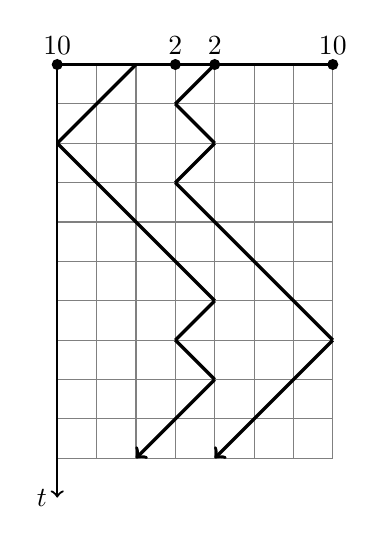
\begin{tikzpicture}
      \draw [help lines,thin,step=5mm] (0,-5.0) grid (3.5,0);
      \draw[thick] (0,0) -- (3.5,0) node [below] {};
      \draw[thick, ->] (0,0) -- (0,-5.5) node [left] {$t$};
      \fill ( 0   , 0) coordinate (c1) circle (2pt) node [above] {10};
      \fill ( 1.5 , 0) coordinate (c2) circle (2pt) node [above] {2};
      \fill ( 2.0 , 0) coordinate (c3) circle (2pt) node [above] {2};
      \fill ( 3.5 , 0) coordinate (c5) circle (2pt) node [above] {10};
      \draw[very thick,- ] ( 1.0, 0  )--(   0,-1.0);
      \draw[very thick,- ] (   0,-1.0)--( 2.0,-3.0);
      \draw[very thick,- ] ( 2.0,-3.0)--( 1.5,-3.5);
      \draw[very thick,- ] ( 1.5,-3.5)--( 2.0,-4.0);
      \draw[very thick,->] ( 2.0,-4.0)--( 1.0,-5.0);
      \draw[very thick,- ] ( 2.0, 0  )--( 1.5,-0.5);
      \draw[very thick,- ] ( 1.5,-0.5)--( 2.0,-1.0);
      \draw[very thick,- ] ( 2.0,-1.0)--( 1.5,-1.5);
      \draw[very thick,- ] ( 1.5,-1.5)--( 3.5,-3.5);
      \draw[very thick,->] ( 3.5,-3.5)--( 2.0,-5.0);
    \end{tikzpicture}
  \end{minipage}
  \begin{minipage}{0.32\hsize}
    \centering
    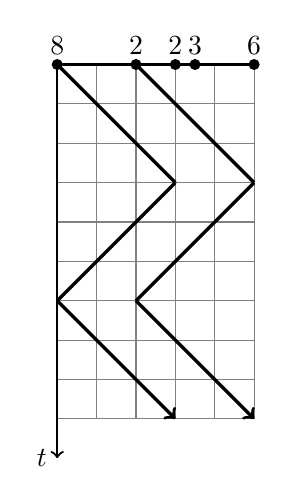
\begin{tikzpicture}
      \draw [help lines,thin,step=5mm] (0,-4.5) grid (2.5,0);
      \draw[thick] (0,0) -- (2.5,0) node [below] {};
      \draw[thick, ->] (0,0) -- (0,-5) node [left] {$t$};
      \fill ( 0   , 0) coordinate (c1) circle (2pt) node [above] {8};
      \fill ( 1   , 0) coordinate (c2) circle (2pt) node [above] {2};
      \fill ( 1.5 , 0) coordinate (c3) circle (2pt) node [above] {2};
      \fill ( 1.75, 0) coordinate (c4) circle (2pt) node [above] {3};
      \fill ( 2.5 , 0) coordinate (c5) circle (2pt) node [above] {6};
      \draw[very thick,- ] ( 0  , 0  )--( 1.5,-1.5);
      \draw[very thick,- ] ( 1.5,-1.5)--( 0  ,-3  );
      \draw[very thick,->] ( 0  ,-3  )--( 1.5,-4.5);
      \draw[very thick,- ] ( 1  , 0  )--( 2.5,-1.5);
      \draw[very thick,- ] ( 2.5,-1.5)--( 1  ,-3  );
      \draw[very thick,->] ( 1  ,-3  )--( 2.5,-4.5);
    \end{tikzpicture}
  \end{minipage}
  \begin{minipage}{0.32\hsize}
    \centering
    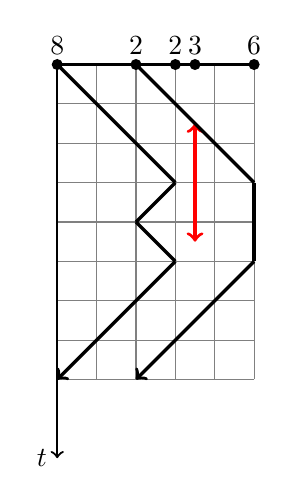
\begin{tikzpicture}
      \draw [help lines,thin,step=5mm] (0,-4) grid (2.5,0);
      \draw[thick] (0,0) -- (2.5,0) node [below] {};
      \draw[thick, ->] (0,0) -- (0,-5) node [left] {$t$};
      \fill ( 0   , 0) coordinate (c1) circle (2pt) node [above] {8};
      \fill ( 1   , 0) coordinate (c2) circle (2pt) node [above] {2};
      \fill ( 1.5 , 0) coordinate (c3) circle (2pt) node [above] {2};
      \fill ( 1.75, 0) coordinate (c4) circle (2pt) node [above] {3};
      \fill ( 2.5 , 0) coordinate (c5) circle (2pt) node [above] {6};
      \draw[very thick,red,<->] (1.75,-0.75)--(1.75,-2.25);
      \draw[very thick,- ] ( 0  , 0  )--( 1.5,-1.5);
      \draw[very thick,- ] ( 1.5,-1.5)--( 1  ,-2  );
      \draw[very thick,- ] ( 1  ,-2  )--( 1.5,-2.5);
      \draw[very thick,->] ( 1.5,-2.5)--( 0  ,-4  );
      \draw[very thick,- ] ( 1  , 0  )--( 2.5,-1.5);
      \draw[very thick,- ] ( 2.5,-1.5)--( 2.5,-2.5);
      \draw[very thick,->] ( 2.5,-2.5)--( 1  ,-4  );
    \end{tikzpicture}
  \end{minipage}
  \end{tabular}
  \caption{巡査の協力が必要な例.
    横軸を点の座標,縦軸を時刻として巡査の軌跡を表す.
    点の上の数値は{\maxIdletime}を表す.
    \ncomment{[あとで図を差し替える]}
    \label{tikz:multiAgentExample2}}
\end{figure}


これらの例は,{\maxIdletime}が異なる場合は巡査の運行を個別に決定するのは難しいということを示唆している.
しかしながら,
地図が{\graphLine}で{\maxIdletime}が一般の場合での{\patProb}の困難性を示すこともできなかった.
そこで,{\maxIdletime}より短い間隔で点を訪問しうることで運行の決定が複雑になる例が存在したことを踏まえて,
ここでは1節で定義した{\timeSpecifiedPatProbDecision}という別種の問題を代わりに考える.



地図が{\graphLine}の場合の{\timeSpecifiedPatProbDecision}は次のようにも記述できる.

\begin{defi}
  $S \subset \Zset \times \Zset$とする.
  任意の$(t_1, x_1), (t_2, x_2) \in S$が
  $\abs{x_1 - x_2} \leq \abs{t_1 - t_2}$を満たすとき,
  $S$は\defword{運行可能}であるという.
  また,分割$\{ P_1, \ldots, P_h \}$が\defword{運行可能}であるとは,
  $P_1, \ldots, P_h$がそれぞれ運行可能集合であることである.
\end{defi}

任意の運行可能集合$S$に対して,
{\graphLine}上の巡査の運行$a$であって,
$S$のすべての元$(t, x)$に対して$a(t) = x$を満たす
(このとき$a$を運行可能集合$S$に対応する運行と呼ぶ)
ものが存在することは簡単に示される.

\begin{timeSpecifiedPatrollingProblemOnLine}
  正の整数$m$と
  $n$個の自然数の組$(q_i, r_i, x_i)_{ i \in \{ 1, \ldots, n \} }$が与えられる.
  集合
  $\{ (q_i k + r_i, x_i) \mid i \in \{1, \ldots, n\}, k \in \Zset \}$を
  $m$個以下の運行可能集合に分割できるか判定せよ.
\end{timeSpecifiedPatrollingProblemOnLine}


{\timeSpecifiedPatProbOnLine}は以下に示す貪欲アルゴリズムにより解くことができる.

まず,地図が{\graphLine}の場合は順序保存運行を考えることができるのと同様に,
順序保存(運行可能)分割も考えることができる.
分割$\mathcal{P} = \{ P_1, \ldots, P_h \}$が順序保存であるとは,
$\mathcal{P}$に対応する運行$A = (a_1, \ldots, a_h)$であって
順序保存なものが存在すること,
あるいは,
\[
  L(t, x)
    := \{ (t', x') \mid
          \abs{x - x'} > \abs{t - t'} \;\textrm{かつ}\; x' < x \}
    = \{ (t', x') \mid {x - x'} > \abs{t - t'} \}
\]
として,
任意の$P_i\ (i \in \{ 1 \ldots, h \})$について,
領域$\bigcup_{(t, x) \in P_i} L(t, x)$に
$P_j\ (i < j)$の点が存在しないことと定義される.

\newcommand{\minpart}{\mathfrak{P}}

$X := \{ (q_i k + r_i, x_i) \mid i \in \{1, \ldots, n\}, k \in \Zset \}$の
任意の順序保存分割のうち一番左の集合は順序保存分割の定義から
$\minpart_1 := \{ (t, x) \in X \mid L(t, x) \cap X = \emptyset \}$の
部分集合となる.
よって,$X$の最小の順序保存分割であって一番左の集合が
$\minpart_1$であるようなものが存在する.
%
同様に,残りの$X \setminus \minpart_1$の最小の順序保存分割であって一番左の集合が
$\minpart_2 :=
  \{ (t, x) \in X \setminus \minpart_1
      \mid L(t, x) \cap X \setminus \minpart_1 = \emptyset \}$であるようなものが存在する.
このように,集合$X$の左側から貪欲に運行可能集合を取り出していく操作を再帰的に繰り返すと,
最小の順序保存分割$\{ \minpart_1, \minpart_2, \ldots, \minpart_h \}$が得られる.
これを$\minpart(X)$と書くことにする.
{\timeSpecifiedPatProbOnLine}の判定は$\card{\minpart(X)} \leq m$が成り立つかの判定をすればよい.

\newcommand{\subsegment}[3]{{#1}_{[#2:#3)}}
以下では,集合$S \subseteq \Zset \times \Zset$に対して
$\subsegment{S}{a}{b} := \{ (t, x) \in S \mid a \leq t < b \}$と定義する.

$q_1, \ldots, q_n$が整数であるので
$X$は時刻(組$(t, x) \in X$の第1要素)について周期的であり,
その周期は$q_1, \ldots, q_n$の最小公倍数$T$となる
(すなわち,任意の整数$k$に対して,
$(t, x) \in \subsegment{X}{kT}{(k + 1)T}$と$(t - kT, x) \in \subsegment{X}{0}{T}$が同値である).
従って,前述の貪欲な分割$\minpart(X)$の各要素
$\minpart_i\ (i \in \{1, \ldots, h \})$も同様に時刻について周期的である
(すなわち,任意の$\minpart_i$と整数$k$に対して,
$(t, x) \in \subsegment{\minpart_i}{kT}{(k + 1)T}$と
$(t - kT, x) \in \subsegment{\minpart_i}{0}{T}$が同値である).
%
よって,
$X$の最小の運行可能分割
$\minpart(X) = \{ \minpart_1, \ldots, \minpart_h \}$の大きさを計算するには,
$\subsegment{X}{0}{T}$の運行可能分割
$\{ \subsegment{\minpart_1}{0}{T}, \ldots, \subsegment{\minpart_h}{0}{T} \}$を計算できればよい.

ここで,$\minpart(\subsegment{X}{0}{T})$と$\minpart(X)$の大きさは
必ずしも一致しないことに注意する必要がある.
前述の貪欲な分割の仕方で集合$S$から左端の運行可能集合
$s' := \{ (t, x) \in S \mid L(t, x) \cap S = \emptyset \}$を取り出すとき,
$s'$の点$(t, x)$の条件は領域$L(t, x)$に$S$の点が存在しないことである.
$X$を$\minpart(X)$へ分割するときと「同じ条件で」$\subsegment{X}{0}{T}$を分割する
(すなわち,$\subsegment{X}{0}{T}$を
$\{ \subsegment{\minpart_1}{0}{T}, \ldots, \subsegment{\minpart_h}{0}{T} \}$%
に分割する)には,
$X' := \{ (t, x) \in X \mid
  (t', x') \in \subsegment{X}{0}{T} \ \textrm{が存在して}\ (t, x) \in L(t', x') \}$%
として$\minpart(X')$を求めればよい.
以下の
有限集合$F$の分割$\minpart(F)$を与える{\setPartitionAlgorithm}
の入力として$X'$を与えればよい.
あとは,出力された分割$\mathcal{P}$の各要素を$[0:T)$に制限すれば
$\subsegment{X}{0}{T}$の分割$\{ \subsegment{\minpart_1}{0}{T}, \ldots, \subsegment{\minpart_h}{0}{T} \}$が得られる.

\begin{setPartitionAlgorithmForTimeSpecifiedProblemOnLine}
  入力を有限集合$F$とする.
  初期値を$\mathcal{P} = \{\}$, $F' = F$とし,
  $F' \neq \emptyset$である限り
  次の\ref{item:alg_step_first}から\ref{item:alg_step_last}を繰り返す.
  \begin{enumerate}
  \item \label{item:alg_step_first}
    $P \gets \{ (t, x) \in F' \mid L(t, x) \cap F' = \emptyset \}$
  \item
    $\mathcal{P} \gets \mathcal{P} \cup \{ P \}$
  \item \label{item:alg_step_last}
    $F' \gets F' \setminus P$
  \end{enumerate}
  $\mathcal{P}$を出力する.
\end{setPartitionAlgorithmForTimeSpecifiedProblemOnLine}

  
\section{Star}
グラフの形状がStarの場合については,
利得か{\timelimit}のいずれかが一般であれば,
{\patrolling}は巡査が1人であってもNP困難であることがわかっている\cite{coene2011charlemagne}.
そこで,ここでは巡査数が一般であって,
利得と{\timelimit}がすべて等しい場合を考える.
%
この場合,非協力警邏問題ではNP困難になることが
Coeneら\cite{coene2011charlemagne}により示されているが,
今回考えている協力警邏問題では多項式時間で解くことができる.
%
これは,
非協力の場合にはうまく分担する方法を見つける必要があるのに対し,
協力警邏の場合には単純で最適な警邏を構成できることが理由となっている.

以下では
% そのような単純な警邏の仕方を示していくが,
{\timelimit}を$Q$とするとき,
「複数人の巡査が間隔$Q$ずつ離れて列を成し巡回する」動き
と「点に1人の巡査が常駐する」という2種類の運行の組合せで
最適な運行が得られることを示す.

% 隣接枝が一定以上長い点は
% 枝の往復にかかる時間が大きくなるため,
% 巡回に含めずに巡査を1人常駐させる方が
% この点の1回あたりの警備にかかる時間を減らすことができる.



\begin{theo}
    \label{theo:StarEqualProfitTimelimit}
    グラフの形状がStarで利得と{\timelimit}がすべて等しい場合,
    {\patrolling}は多項式時間で解くことができる.
\end{theo}


\begin{proof}[証明]

    巡査数を$m$, 全頂点の{\timelimit}を$Q$, 
    頂点$v_i (i \in \mathset{1,\ldots, n})$に隣接する枝を$e_i$, その長さを$d_i$とする.
    枝の長さは$d_1 \leq d_2 \leq \cdots \leq d_n$であるとする.

    まず,
    すべての頂点の利得と{\timelimit}が等しいので,枝の短い頂点から選べばよいことが分かる.
    実際,ある警邏において警備している頂点$v_i$と警備していない頂点$v_j$であって
    隣接枝$e_i$, $e_j$の長さが$d_i > d_j$となっているようなものがあったとき,
    $v_j$を訪問していた時刻に代わりに$v_i$を訪問するようにすべての巡査の動きを変えることができる.




    まず,$d_i > Q/2$であるような頂点$v_i$は,警備するならば巡査が1人常駐するとしてよい.
    これは次のように示される.
    %
    (i)ある運行において$v_i$が1人の巡査$s$により単独警備されるとすると,
    $v_i$を訪問してから別の頂点$v_j$を訪問して再び$v_i$に戻ってくるには$2d_i$以上の時間がかかり
    $2d_i > Q$より$v_i$が警備できなくなってしまうため$v_i$以外の頂点を警備することができないので
    $v_i$のみを警備すればよく,これは$v_i$に常駐すれば十分である.
    %
    (ii)もし$v_i$が2人以上の巡査により警備されるとすると,
    ある巡査$s_a$が時刻$t_a$に$v_i$を訪問してから時間$Q$以内の時刻$t_b$に
    別の巡査$s_b$が$v_i$を訪問するという状況が発生するが,
    $s_a$が枝
    $s_b$は端点$v_i$を含む枝$e_i$上のある点に同時に存在するような時刻が
    $s$が
    $s$は$s'$とすれ違うことなく$v_i$以外の頂点を訪問



    2人の巡査がすれ違う動きは互いに動きを交換して引き返す動きに変換しているとすると
    $s$と$s'$が枝$e_i$上で1度以上すれ違わない限り$s'$が$v_i$を訪問するときには$s$も
    $v_i$を訪問しているので,
    $v_i$は$s$のみにより警備できており,$s$も$v_i$以外を警備していない動きとなる.



    よって,あとは隣接している枝の短い頂点から何個の頂点を選べるかを計算できればよい.
    %
    はじめに,頂点を枝の長さの昇順でソートし,枝の短いものから順に$v_1,v_2, \ldots, v_n$とする.
    これらを枝の長さが$Q/2$以下のグループ$V_1 = \mathset{v_1, \ldots, v_k}$と
    それ以外のグループ$V_2 = \mathset{ v_{k + 1}, \ldots, v_n }$に分ける.
    $V_2$の頂点は,$V_1$の全頂点を$m - 1$人以下の巡査により警備できる場合のみ,
    残りの巡査の人数分$V_2$の頂点を選び1人ずつ巡査を常駐させることで警備すればよいので,
    まず$V_1$のすべての頂点を警備できる最小の巡査数$m'$を求める必要がある.

    $m' \leq m$であれば利得(警備できる頂点数)は$k + (m - m')$となる.
    $m' > m$であれば$V_1$のうち

\end{proof}


  \chapter{{\graphUnit}}
\label{chapter: unit}

\ref{chapter: introduction}章で述べたように
{\graphUnit}は{\graphStar}の特殊な場合とみなせるため,
全点の利得と{\maxIdletime}が等しい場合,{\PPProfit}は
定理\ref{theo:StarUnaryProfitAndIdletime}により多項式時間で解くことができる.
ここでは,
{\graphUnit}で
全点の{\maxIdletime}が等しい場合の{\PPProfit}が(利得が異なっていても)多項式時間で解ける
ことを示す(定理\ref{theo:UnitUnaryIdletime}).

{\maxIdletime}が一般の場合については
多項式時間アルゴリズムやNP困難性を示すのが難しかったため,
\ref{chapter: line}章で扱った{\timeSpecifiedPPProfit}を再び考える.
地図が{\graphUnit}の場合は{\timeSpecifiedPPProfit}がNP困難になることを示す
(定理\ref{theo:UnitExacIdletimeNPhard}).



\section{全点の{\maxIdletime}が等しい場合}
\label{section: UnitUnaryIdletime}

\begin{theo}
  \label{theo:UnitUnaryIdletime}
  地図が{\graphUnit}で全点の{\maxIdletime}が等しい場合,
  {\PPProfit}は(利得,巡査数が一般であっても)
  多項式時間で解くことができる.
\end{theo}

\begin{proof}
  {\maxIdletime}を$q$とし,各辺の長さを$d$とする.
  {\graphUnit}は{\graphStar}の特殊な場合であるから,
  補題\ref{lemm:StarConditionOfGuarding}が適用できる.
  すなわち点集合$W$が$m$人で警邏できるためには,
  式\eqref{equation: star bound}が$d _v = d / 2$で成立つこと,
  つまり$W$に属する点の個数$\card{W}$が
  \begin{equation}
    \card{W} \cdot \min (d, q) \leq m q
  \end{equation}
  を満すことが必要十分である.
  したがって,利得の大きい順に
  $\lfloor m q / \min (d, q) \rfloor$個の点を選んだものが最適の$W$である.
\end{proof}

{\graphStar}で全点の{\maxIdletime}が等しい場合は,
警邏できる点の最大数が式\eqref{equation: star bound}で与えられることから,
利得が等しい場合は枝の短いものから選べばよく(定理\ref{theo:StarUnaryProfitAndIdletime}),
枝の長さが等しい場合は利得の大きいものから選べばよい(定理\ref{theo:UnitUnaryIdletime})
というようにまとめることができる.




  \section{{\maxIdletime}が一般の場合}
\label{section: UnitArbitraryIdletime}

\ref{chapter: star}章冒頭で述べた通り,
地図が{\graphStar}の場合については,
{\maxIdletime}が一般の場合は
{\PPProfit}は巡査が一人であってもNP困難であった\cite[Theorem~6]{coene2011charlemagne}.
このNP困難性の証明では
辺の長さが異なる{\graphStar}の地図を用いていた.
{\graphUnit}は{\graphStar}の辺の長さがすべて等しい場合であるため,
この方法によるNP困難性の証明ができない.
{\graphUnit}で{\maxIdletime}が一般の場合は
多項式時間アルゴリズムやNP困難性の証明が難しかったため,
{\graphLine}のときのように{\timeSpecifiedPPProfit}を代わりに考える.


地図$(U, V)$が{\graphUnit}で
各点$v_i \in V$の{\exactTime}が$(q_i, r_i)$のとき,
巡査一人で$V$の全点を定時訪問できるかどうかは次のように多項式時間で判定できる.
%
辺の長さを$d$とすると,
$V$の異なる2点$i, j$の間の移動には時間$d$を要することから,
その両方を定時訪問できるためには,
訪問すべき時刻どうしがすべて$d$以上離れていること,すなわち
任意の整数$k, l$に対して$\abs{(q_i k + r_i) - (q_j l + r_j)} \geq d$%
が成り立つことが必要十分である.
$g$を$q_i$と$q_j$の最大公約数として,
これは任意の整数$n$で
$\abs{(r_i - r_j) + gn} \geq d$%
が成り立つことに等しいので,
$r_i, r_j$をそれぞれ$g$で割った余りを$r_i', r_j'$として
$\abs{r_i' - r_j'}$,
$\abs{r_i' - r_j' + g}$,
$\abs{r_i' - r_j' - g}$%
のいずれも$d$以上となることに等しい.
%
全点を定時訪問可能かどうかは,この条件を$V$のすべての2点について確かめればよい.

全点を定時訪問可能か判定する問題は多項式時間で解けるのに対し,
{\timeSpecifiedPPProfit}では次が成り立つ.


\begin{theo}
  \label{theo:UnitExacIdletimeNPhard}
  地図が{\graphUnit}のとき,
  {\timeSpecifiedPPProfit}は巡査が一人で全点の利得が等しい場合であってもNP困難である.
\end{theo}
\begin{proof}
  % 最大独立集合問題において,
  % 無向グラフが与えられたときに独立点集合で最大のものを求めるが,
  % 間に辺の存在する2点の両方を選ぶことはできないという制約を,
  % {\PPProfit}において2点のどちらか一方しか警邏できないという制約に変換する.
  NP困難であることが知られている最大独立集合問題からの帰着による.
  最大独立集合問題は,無向グラフが与えられたとき,
  どの二点間にも辺が存在しないような頂点集合(独立集合)のうち
  頂点の個数が最大のものを求める問題である.

  \newcommand{\primenum}[2]{p_{{#1}{#2}}}
  最大独立集合問題の入力として
  点集合$[n] = \{1, \ldots, n\}$,
  辺集合$E$のグラフ$G$が与えられたとする.
  同じ大きさの点集合$V$をもち,利得をすべて$1$,辺の長さをすべて$1$とした
  {\graphUnit}の地図$M = (U, V)$を考える.
  各点$v_i \in V$の{\exactTime}$(q_i, r_i)$を次のように定める.
  まず,$n(n - 1)/2$個の相異なる素数$\primenum{i}{j}\ (1 \leq i < j \leq n)$を用意する.
  $i > j$に対して$\primenum{i}{j}$と書くときは$\primenum{j}{i}$を指すことにする.
  各$i \in [n]$について,
  \begin{equation}
    q_i = \prod_{j \in [n] \setminus \{i\}} \primenum{i}{j}
  \end{equation}
  とし,
  $r _i$をすべての$j \in [n] \setminus \{i\}$に対して
  次を満たすように定める.
  \begin{equation}
    \label{equation: residues}
    r _i
    \equiv
    \begin{cases}
      1 & \text{$(i, j) \notin E$かつ$i > j$のとき} \\
      0 & \text{それ以外のとき}
    \end{cases}
    \pmod{\primenum{i}{j}}
  \end{equation}
  そのような$r _i$は
  中国剰余定理より($q _i$の剰余として一意に)存在する.

  $V$の異なる2点$v_i, v_j$の間の移動には時間$1$を要することから,
  その両方を定時訪問できるためには,
  $q_i$と$q_j$の最大公約数$\primenum{i}{j}$について
  $\abs{(r_i - r_j) + \primenum{i}{j} k} \geq 1$%
  が任意の整数$k$で成り立つことが必要十分である.
  $r_i, r_j$が整数なので,これは
  $r_i - r_j$が$\primenum{i}{j}$の倍数でないこと,
  つまり$r_i \not\equiv r_j \mod \primenum{i}{j}$に同値である.
  %
  $r_i$の決め方\eqref{equation: residues}から,
  これは$(i, j) \notin E$に同値である.
  以上より,
  $(i, j) \in E$と$M$の2点$v_i, v_j$を両方定時訪問することができないこと
  が同値となるため,
  $M$の最大の警邏可能な点部分集合は$G$の最大独立集合となることがわかる.

  また,
  $k$番目に小さい素数を$P_k$と書くと,$k \geq 6$について
  $P_k < k( \ln k + \ln\ln k )$が成り立つ\cite{dusart1999k}ので,
  $n(n - 1)/2$個の素数の列挙は$n$の多項式時間でできる.
\end{proof}

なお,
地図が{\graphUnit}で巡査が一人かつ全点の利得が等しい場合は
全点を定時訪問可能か判定する問題は本節冒頭で示した通り多項式時間で解けるので,
整数$N$が与えられたとき定時訪問可能な部分集合であって大きさが$N$以上のものが存在するか判定する問題はNPに属する.
この問題は定理\ref{theo:UnitExacIdletimeNPhard}よりNP困難なのでNP完全である.




\section*{定期訪問の場合}

定理\ref{theo:UnitExacIdletimeNPhard}では,
点$v_1, \ldots, v_n$を{\exactTime}$(q_1, r_1), \ldots, (q_n, r_n)$に訪問せねばならないという{\timeSpecifiedPPProfit}がNP困難であることを示したが,
$r_1, \ldots, r_n$は与えられず$q_1, \ldots, q_n$のみが指定される
次のような問題も考えることができる.

\begin{intervalSpecifiedPatrollingProblem}
  巡査の人数$m$と地図$(U, V)$および
  各点の{\exactInterval}$(q_1, \ldots, q_n)$が与えられる.
  $m$人の巡査により$V$の全点を定期訪問できるか判定せよ.
  ただし,点$v$を\defword{\exactInterval}$q$で\defword{定期訪問}するとは,
  非負整数$r\ (0 \leq r < q)$が存在して
  $v$を{\exactTime}$(q, r)$で定時訪問することである.
\end{intervalSpecifiedPatrollingProblem}

巡査が一人の場合の{\timeSpecifiedPP}では
各点を訪問すべき時刻が完全に定められていたため,
全点を警邏できるかどうかは
任意の2点の両方を警邏できるかを判断すれば必要十分であった.
一方,
{\intervalSpecifiedPP}では
各点を訪問すべき時刻は間隔のみしか定められていないため,
同様の判断の仕方ができない.
実際,
地図が{\graphUnit}で二点間距離が$1$の場合の
{\intervalSpecifiedPP}は
CampbellとHardin\cite{campbell2005vehicle}がDVMPDと呼んでいる問題と同じものであり,
巡査が一人であってもNP困難である\cite[Theorem~4]{campbell2005vehicle}.
% 河村と添島も
% 巡査が一人の場合であってもNP困難であることを示している\cite[Theorem~20]{kawamura2015simple}.


  \bibliographystyle{jplain}
  \bibliography{bunken}
\end{document}
